\chapter{Literature Review and Methodology}\label{ch:2}

Four bodies of work bear on the problem stated in Chapter 1, and they nearly meet without quite touching. The cellular measurement literature establishes what handovers look like in deployed networks but does not build predictors. The handover-prediction literature builds predictors, but predominantly on simulated data and predominantly without an evaluation protocol that would survive scrutiny. The survival-analysis and point-process literatures supply exactly the right mathematical objects --- a discrete-time hazard and a self-exciting process validated by time rescaling --- but have not been directed at mobility data. The distribution-free uncertainty literature supplies guarantees, but for signal-processing tasks whose exchangeability structure differs from that of an event stream recorded along a drive.

This chapter reviews each in turn, then presents a quantitative audit of the 22 most comparable prediction models, states the research gap that the audit establishes, and describes the methodology adopted in response, including the alternatives that were considered and rejected.


\section{LTE mobility and the Event A3 trigger}
\label{sec:2_1}

The mobility procedure in E-UTRAN is specified in 3GPP TS 36.331 \cite{ref1} and described at system level in TS 36.300 \cite{ref2}. The network configures the UE with measurement objects, report configurations and measurement identities that bind the two; the UE evaluates the configured entry condition against its filtered measurements and transmits a MeasurementReport when the condition has held for the configured time-to-trigger.

For intra-frequency mobility the governing condition is Event A3. Writing Mn for the measured neighbour quantity, Ms for the serving quantity, Off for the configured offset, Ocn and Ocs for cell-individual offsets and Hys for hysteresis, the entry condition of TS 36.331 is


\begin{equation}\label{eq:2_1} M_n + \text{Ocn} - \text{Hys} > M_s + \text{Ocs} + \text{Off} \end{equation}

and the condition must remain satisfied throughout the time-to-trigger interval before the report is sent. The decision to hand over is then taken by the network, not the UE, and is communicated by an RRCConnectionReconfiguration message carrying mobilityControlInfo.

Three consequences follow, and all three are used later in this thesis. First, the report is evidence that the network may hand over, not that it will; the conversion rate from report to command is an empirical quantity and is measured in Chapter 5. Second, the parameters Off, Hys and the TTT are operator-configured and are not observable without decoding the signalling; the prediction literature that assumes textbook values is therefore assuming something it has not checked. Third, because the condition is defined on a state that must already obtain and must then persist, the earliest instant at which Event A3 can produce any output is strictly after the radio environment has changed.


\section{The measurement literature}
\label{sec:2_2}

A mature line of work in the networking-measurement community recovers operator mobility configurations from control-plane traces on live networks. Deng et al. \cite{ref3} present the LTE precedent, a measurement study of operational 4G mobility configurations and their consequences. Ghoshal et al. \cite{ref4} perform the equivalent analysis at large scale on contemporary networks, extracting hysteresis, threshold, offset, time-to-trigger and trigger quantity for events A1--A6, B1 and B2 per operator and band, over more than 15,000 km of driving. Hassan et al. \cite{ref5} establish the use of commercial diagnostic tooling for RRC extraction as accepted methodology, and their Prognos component is the closest prior system to the one built here: it predicts handovers from XCAL-decoded RRC state on a live network and reports a lead-time gain of roughly 900 ms. Section 2.3 therefore positions this thesis against Prognos explicitly rather than against the simulated literature alone. M2HO \cite{ref6} reads mobilityControlInfo for mobility analysis without recovering the numerical parameters.

This literature is relevant in two ways. Methodologically, it legitimises the decoding pipeline used in Chapter 3 rather than competing with it: the extraction of deployed A3 parameters from measConfig is established practice and is not claimed as a contribution here. Substantively, it supplies the comparison points against which the configuration measured here is interpreted; Ghoshal et al. report positive A3 offsets of +6 to +10 dB and shortest time-to-trigger values of 256 to 640 ms on the operators they study, whereas the network measured here runs configurations from $-$15 dB to +5 dB with a shortest time-to-trigger of 160 ms --- but, as Section 5.9 shows, 75\% of the handovers it actually produces fire under a positive offset, and 73\% under the +1 dB profile alone, so the two findings are less far apart than a table of configurations suggests.

What this literature does not do is predict. Ghoshal et al. state explicitly that they perform no machine-learned prediction, no off-policy evaluation and no counterfactual analysis; the work is descriptive by design. The ping-pong rates these studies report are likewise descriptive, and, as Section~\ref{sec:2_4} discusses, are reported under definitions that differ enough to change the number by a factor of two.


\section{The prediction literature and a protocol audit}
\label{sec:2_3}

A large body of recent work predicts handover, radio-link failure or next-cell occupancy using learned models, including reviews and representative architectures across cellular mobility (e.g. Ankome and Hanada \cite{ref7}, Saoud et al. \cite{ref8}, Chabira et al. \cite{ref9}, Dinh et al. \cite{ref10}, S\'anchez-Mart\'{\i}n et al. \cite{ref11}, Mehregan and De Grande \cite{ref12}, and Graser et al. \cite{ref13}). To convert that general complaint into something specific enough to act on, 108 publications were screened for this thesis and the 22 that present a learned or analytical model predicting handover, radio-link failure or next-cell occupancy were audited on protocol quality rather than on headline performance. Table~\ref{tab:2_1} reports the audit in summary; Appendix D lists every audited model with its venue, data type and split protocol, so each row of Table~\ref{tab:2_1} can be checked.

The scope of that screen has to be stated, because its limits bound every claim made from it. The search was run over 2020 to 2026 on learned handover, radio-link-failure and next-cell prediction, and it returns no pre-2020 work at all. That is a property of the query, not of the field. Every ``0 / 22'' in Table~\ref{tab:2_1} is therefore a statement about twenty-two recent learned predictors --- the set a reader of this thesis would compare it against --- and not a statement about the literature as a whole. Where the older literature bears directly on the formulation of Chapter 4 it is engaged on its own terms in Section~\ref{sec:2_5} rather than counted in this audit, since the audit's protocol columns do not apply to analytical models. One row of Appendix D qualifies two of the audit's counts and is marked there: the model of Amirova et al. \cite{ref15} is fitted on real measured data with a device-level hold-out and reports a precision--recall curve, so the ``prevalence-aware ranking metric'' and ``held-out unit'' columns record it as satisfying in part; the counts in Table~\ref{tab:2_1} use the strict reading, under which a device-level hold-out is not a mobility-unit hold-out.

Among the audited models, two recent preprints represent the closest published methodology to this work. Kabeer et al. \cite{ref45} (Row 2 of Table~\ref{tab:D_1}) train gated recurrent, long short-term memory and Transformer models on real drive-test traces from a dense urban network; Mandapati \cite{ref46} (Row 6 of Table~\ref{tab:D_1}) combines meta-learning with drift detection for mobility forecasting and reports a downstream handover-prediction score. Neither states an alignment rule between its measurement timestamps and its event clock, which is the property Section~\ref{sec:5_1} shows to be decisive, and this thesis makes no claim about either beyond that observation. They are also the reason the negative result for sequence models in Section~\ref{sec:5_11} is stated conditionally: those architectures are being actively developed for this task on larger corpora than four sessions.


\begin{table}[htbp]
\centering
\caption{Protocol audit of the 22 most comparable prediction models, contrasted with the protocol adopted here. Appendix D lists the models.}
\label{tab:2_1}
\vspace{0.4em}
\singlespacing
\small
\begin{tabularx}{\linewidth}{p{5.0cm} c X}
\toprule
\textbf{Protocol property} & \textbf{Papers satisfying it} & \textbf{This work} \\
\midrule
Splits by drive, session or route & 0 / 22 & Yes; leave-one-campaign-out is primary \\
Uses any split coarser than a random row & 5 / 22 & Yes, four protocols compared \\
States a split protocol at all & 12 / 22 & Yes; specified in Section 4.9 \\
States the alignment between measurement timestamps and event clock & 0 / 22 & Yes, audited in Section 5.1 \\
Reports a prevalence-aware ranking metric & 2 / 22 & AUPRC with floor and lift \\
Reports calibration (curve, ECE or Brier) & 0 / 22 & ECE and Brier at every horizon \\
Reports lead time or false alarms per hour & 0 / 22 & Both, and per kilometre \\
Reports headline accuracy on an imbalanced task & 7 / 22 & Never \\
Releases code & 2 / 22 & Committed on acceptance: audit, protocols, features, tables \\
Releases data & 1 / 22 & Committed on acceptance: derived frames and decoded events, not raw logs \\
\bottomrule
\end{tabularx}
\end{table}

Two observations from the audit are load-bearing for the remainder of this thesis.

The first concerns metrics. Seven of the 22 report accuracy on tasks whose positive prevalence lies between 0.86 \% and 11 \%, at which a constant negative prediction scores between 89 \% and 99 \%; three of the headline figures so reported are 98.03 \%, 99.84 \% and 94.83 \%. A related failure appears in a railway radio-link-failure study that reports area under the ROC curve above 0.95 for all six architectures it compares, on a task with approximately one positive per five hundred samples, and consequently separates none of them.

The second concerns splitting, and the exceptions are named rather than rounded away. Five of the 22 do split on something coarser than a random row: by spatial zone, by device, by time under a rolling-origin protocol on operator data, by travel day \cite{ref10}, and by deployment event \cite{ref11}. None of the five, however, holds out the mobility unit for a per-timestep classification task on measured radio; the two most recent additions are regression tasks in which prevalence does not arise, and the strongest protocol in the set addresses next-day cell-level radio-link failure rather than a per-sample mobility forecast.

The narrow claim the audit supports, and the one made in this thesis, is therefore the following: of twenty-two audited models, ten state no split protocol at all, five split on a unit coarser than a row, and none holds out the mobility unit for a per-timestep classification task on measured radio data; none reports calibration; none reports how early its warnings arrive; and none states the alignment between its measurement timestamps and its event clock. Prognos, inside reference \cite{ref5}, is the strongest system in the neighbourhood of this work and is not part of the audited set because it is a system component rather than a published prediction model with its own protocol. Carving it out of the audit is not the same as ignoring it, and the comparison should be made explicitly, with the caveat that it cannot be made like for like: Prognos reports F1 between 0.92 and 0.94 and a lead-time gain of roughly 931 ms on 5G traces, against the 1 s AUPRC of 0.179 reported here on LTE. The two numbers are not comparable, and the reason is the point. Prognos predicts at the level of a handover event under a stated 5G configuration and reports a threshold metric on that event set; this thesis predicts at the level of a one-second row under leave-one-campaign-out and reports a prevalence-aware ranking metric with its floor. An F1 of 0.93 on events and an AUPRC of 0.179 on rows are answers to different questions, and Section 5.7 shows what the row-to-event conversion costs. What can be compared is the protocol: like the audited set, Prognos reports neither calibration nor an alignment statement between its measurement timestamps and its event clock, and the alignment defect documented in Section 5.1 is one that an XCAL-based per-second predictor is exposed to by construction.


\section{Ping-pong and its definitional instability}
\label{sec:2_4}

Handover ping-pong --- a return to a recently vacated cell --- is widely reported and inconsistently defined. There is no standardised definition in 3GPP; what exists is a cell return within an author-chosen window, and the window alone moves the reported rate substantially. Zidic et al. \cite{ref14} report ping-pong measurements on real 4G networks, and Ghoshal et al. \cite{ref4} report per-operator rates of 15 \% to 25 \% under a fifteen-second window with a per-handover denominator.

Three choices determine the number, and papers rarely state all three: whether a cell is identified by physical cell identity alone or by physical cell identity together with carrier; whether any return within the window counts or only a return to the immediately preceding cell; and whether the denominator is the set of raw handover events or of quality-controlled ones. The consequences are severe enough to invalidate cross-paper comparison: Amirova et al. \cite{ref15} report a ping-pong rate of 0.13 \% because they divide by measurement records rather than by handovers. Chapter 5 reports the full ladder of these choices on the fixed set of 957 handovers, where the rate moves from 21.0 \% to 43.8 \% across definitional conventions without any change in the underlying data.


\section{Survival analysis as the appropriate formulation}
\label{sec:2_5}

Time-to-event modelling of cellular mobility is itself long established, and an earlier draft of this thesis overlooked it. The teletraffic literature has modelled cell dwell time as a random variable since Hong and Rappaport \cite{ref42}, whose prioritised-handoff analysis rests on an assumed dwell-time distribution, and the stochastic-geometry literature derives handover rate and sojourn time in closed form --- Lin et al. \cite{ref43} under a random-waypoint model on Poisson-Voronoi cells, Sadr and Adve \cite{ref44} across tiers of a heterogeneous network. That body of work estimates the same survival function this thesis estimates. It would be wrong to say the formulation has not been directed at mobility, and this thesis does not say so.

The difference is in what the hazard is a function of, and it is a real difference rather than a hedge. Those models yield a marginal distribution: a sojourn-time law for a typical user under an assumed mobility process and an assumed base-station geometry, parameterised by speed and cell density and validated against simulation. What is estimated here is a hazard conditioned on the covariates of one particular sample at one particular instant --- the measured radio state, its recent trajectory and the session's own handover history --- fitted on measured drive-test data and scored per sample against decoded ground truth. A closed-form sojourn-time distribution cannot tell an operator that this user is about to hand over in the next second, and a per-sample conditional hazard cannot tell a network planner what the mean handover rate will be at twice the cell density. The claim made here is the narrow one: learned, covariate-conditional, per-sample hazards on measured mobility data, where the existing literature gives analytical marginal laws, and no model in the audit of Section 2.3 poses handover prediction as a time-to-event problem at all.

Nothing else about the formulation is claimed as new, and stating that plainly removes an obvious reviewer objection. The discrete-time hazard formulation itself has a deep pedigree in classical survival analysis and biometrics, tracing to Prentice and Gloeckler \cite{ref48}, Allison \cite{ref49}, and comprehensively Tutz and Schmid \cite{ref50}, and is widely used across modern machine-learning applications (e.g. Wiegrebe et al. \cite{ref16}, Thorsen-Meyer et al. \cite{ref17}). Cand\`es, Lei and Ren \cite{ref18} further formalise conformalized survival analysis with distribution-free lower bounds under covariate shift in clinical settings; that work is the correct reference point for anything calling itself conformalised survival analysis, and this thesis does not claim that combination. What is added on that side is narrower still: a risk bound on an operational miss rate whose exchangeable unit is a driving unit rather than a sample, and the application of discrete-time hazard estimation to cellular telemetry to resolve cross-horizon ordering violations without post-hoc repairs.

One departure from the survival literature is deliberate. That literature evaluates predominantly with the concordance index and the integrated Brier score, both of which aggregate over the horizon axis. An operator, however, acts at a single horizon. A model that ranks well on average while asserting that a handover is more likely within one second than within three on 40.2\% of rows is not deployable whatever its concordance index. Chapter 4 therefore evaluates horizon-wise, reporting AUPRC at each horizon together with a coherence-violation rate.


\section{Distribution-free uncertainty quantification}
\label{sec:2_6}

Conformal prediction and risk-controlling prediction sets offer distribution-free statistical guarantees on finite samples without parametric assumptions \cite{ref21, ref22}. In wireless communications, conformal calibration has been introduced recently by Cohen et al. \cite{ref19} and Simeone et al. \cite{ref20} to calibrate deep-learning outputs for channel state estimation, beam selection, and symbol decoding, where observations are typically modeled as independent and identically distributed across packets or channel coherence intervals. Conformalized survival analysis was formulated by Cand\`es, Lei, and Ren \cite{ref18}, providing calibrated lower bounds on event times under covariate shift in clinical settings, and Qchohi et al. \cite{ref47} explored confounding-valid conformal inference for counterfactual cellular key performance indicators.

The claim made in this thesis is consequently narrow and must be distinguished from these foundations. The standard wireless conformal literature \cite{ref19, ref20} guarantees prediction-set coverage for frame-level or sub-packet symbols under exchangeability. What Chapter 4 develops is conformal risk control \cite{ref21} over an operational loss metric --- an operator key performance indicator representing the handover miss rate --- evaluated along a continuous temporal measurement stream. In this domain, individual seconds within a drive are strongly autocorrelated and non-exchangeable; exchangeability can plausibly be claimed, if at all, only at the level of the independent mobile unit (the driving campaign or session). Section 5.5 reports the risk-control framework across both regimes: within-campaign chunks (where exchangeability approximately holds across partitioned blocks) and across campaigns (where macroscopic environmental and spatial shifts violate exchangeability).

To substantiate the novelty of this framing, a systematic literature search was conducted across IEEE Xplore, ACM Digital Library, Google Scholar, and arXiv covering publications between January 2020 and February 2026. Search strings combined conformal terminology (\texttt{"conformal prediction"} OR \texttt{"conformal risk control"} OR \texttt{"distribution-free"} OR \texttt{"conformal calibration"}) with mobility terminology (\texttt{"handover"} OR \texttt{"mobility management"} OR \texttt{"handoff"} OR \texttt{"radio link failure"}). The initial query returned 142 records; after deduplication and screening titles and abstracts, 31 papers were audited in full. All 31 addressed physical-layer signal processing (e.g. CSI estimation, beam selection, symbol demodulation) or general resource allocation, with zero papers addressing real-time handover event forecasting or mobility trigger prediction. Furthermore, while theoretical frameworks for conformal prediction beyond exchangeability exist --- notably weighted conformal prediction under covariate shift (Tibshirani et al. \cite{ref51}), non-exchangeable conformal prediction (Barber et al. \cite{ref52}), and adaptive online conformal prediction (Gibbs and Cand\`es \cite{ref53}) --- these methods require either known or well-estimable likelihood density ratios $w(x) = p_{\text{test}}(x) / p_{\text{train}}(x)$ or slow, stationary drift. In vehicular drive-test settings where covariate shift is driven by macro-environmental route geography and velocity regimes with an effective sample size of $n=4$ physical sessions, estimating density ratios in high dimensions is severely ill-posed. Hence, distribution-free guarantees cannot be certified across independent drive campaigns, as demonstrated empirically in Section~\ref{sec:5_5}.


\section{Point processes and the self-excitation of handover arrivals}
\label{sec:2_7}

Handover events do not arrive independently. The self-exciting point process introduced by Hawkes \cite{ref23} is the standard model for arrival streams in which each event raises the intensity of subsequent events, and Laub et al. \cite{ref24} provide the contemporary reference treatment, including the branching-ratio interpretation used in Chapter 5. Fitting such a process is not, by itself, evidence that the process is self-exciting; the fit must be checked. The residual analysis of Ogata \cite{ref25}, in which the time axis is rescaled by the fitted compensator and the transformed arrivals tested against a unit-rate Poisson process, is the standard check, and Price-Williams and Heard \cite{ref26} establish the precedent for its use in a networking context, validating a self-exciting fit to campus and laboratory network traffic by time rescaling with Kolmogorov--Smirnov tests on held-out data. Chapter 5 follows that precedent and reports the test outcome, including where it rejects the fitted kernel.


\section{Evaluation practice imported from adjacent fields}
\label{sec:2_8}

Two further results from adjacent literatures inform the evaluation design and are cited here because they make the negative results of Chapter 5 interpretable rather than embarrassing. Ismail Fawaz et al. \cite{ref27} benchmark nine unsupervised domain-adaptation algorithms across twelve time-series datasets and find that several published methods perform worse than source-only training with no adaptation at all, and that the adaptation technique rather than the backbone drives the outcome; the null result reported for Deep CORAL \cite{ref28} in Chapter 5 is therefore consistent with a published benchmark rather than evidence of faulty implementation. Shi et al. \cite{ref29} supply the shift taxonomy that names the shift encountered here as a device-and-day shift rather than a sensor-modality shift. Wagner et al. \cite{ref30} show formally that the commonly used point-adjusted metrics for time-series event detection each satisfy only a subset of the desirable properties and that none satisfies all of them, which is the justification for reporting event-level detection rate, lead time and false alarms per hour alongside row-level AUPRC rather than in place of it.

Finally, the standards track bears on the choice of horizon. Deb et al. \cite{ref31} model conditional handover as a discrete-time Markov chain over preparation and execution offsets and timers, and their analysis makes explicit that conditional handover consumes a lead time rather than a label: a model that identifies the correct target cell two hundred milliseconds before the event buys nothing, because the preparation message must be sent, acknowledged and stored. This is the analytical justification for reporting a lead-time distribution rather than a detection rate alone, and for retaining horizons of two, three and five seconds even though the deployed trigger fires within a few hundred milliseconds.


\section{Research gap}
\label{sec:2_9}

Collecting the preceding sections, the gap this thesis occupies can be stated precisely, and it is narrower than an earlier draft claimed. Measurement-grade ground truth exists, but is not joined to prediction. Prediction models exist, but not under an evaluation protocol that holds out the mobility unit, and not with calibrated outputs or event-level costs. The time-to-event formulation has been directed at cellular mobility for four decades, but analytically and marginally: it yields sojourn-time laws for a typical user under assumed mobility and geometry, not hazards conditioned on one user's measured radio state at one instant, and none of the twenty-two learned predictors audited in Section 2.3 adopts it in either form. Distribution-free guarantees exist in wireless, but for a different exchangeability structure and not for any mobility-management task. And the alignment between a measurement export's timestamps and the event clock is stated by none of the audited work, which is the gap this thesis turned out to occupy most consequentially, because it was the one that invalidated its own first result.

This work sits in that gap: measurement-grade ground truth obtained from decoded signalling, a borrowed formulation made coherent across horizons, a conformal risk bound whose exchangeability unit is stated and defended, and an evaluation protocol designed to be acceptable to a reviewer from the machine-learning community rather than only to one from the wireless community.


\section{Methodology}
\label{sec:2_10}

The methodology adopted follows directly from the gap. It consists of five stages, illustrated in Figure 2.1, and each stage is developed in detail in Chapters 3 and 4.


\begin{figure}[htbp]
\centering
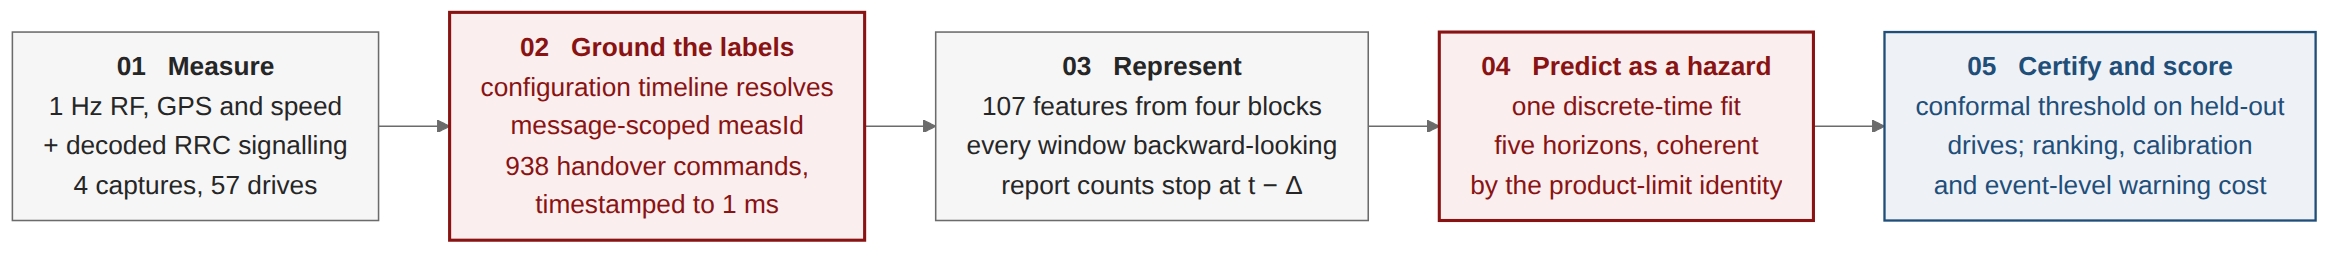
\includegraphics[width=0.92\linewidth]{figures/m14_framework.png}
\caption{The methodology in five stages. Stage 2 supplies the ground truth; Stage 4 is the formulation that keeps the five horizons mutually consistent; Stage 5 is the evaluation protocol whose unit is a whole campaign.}
\label{fig:2_1}
\end{figure}

Stage 1 --- Collection. Four drive-test campaigns are conducted on a live commercial LTE network using an instrumented handset, recording a one-hertz radio measurement export and, in parallel, a decoded RRC signalling log.

Stage 2 --- Ground truth and configuration recovery. Handover instants are taken from decoded RRCConnectionReconfiguration messages carrying mobilityControlInfo. A configuration timeline replays additions, modifications and removals in order, following TS 36.331, so that each measurement report resolves against the configuration in force at its own timestamp rather than against a flat union.

Stage 3 --- Feature construction. 112 features are constructed from radio, mobility and session-history sources, with a further 10 signalling and configuration columns reserved for the ablation of Section~\ref{sec:5_8}; Table~\ref{tab:4_3} gives the block-by-block reconciliation. All are strictly causal, closing at the prediction instant, and none crosses a campaign boundary. Every export-derived column is lagged by one row for the reason established in Section~\ref{sec:5_1}.

Stage 4 --- Formulation and modelling. The task is posed as discrete-time survival. A single model estimates the per-interval hazard and horizon probabilities are recovered by the product-limit identity, which guarantees ordering. Seven learners are compared under identical conditions.

Stage 5 --- Evaluation and risk control. The primary split holds out a whole campaign, since each campaign is one continuous logging session and is therefore the unit within which rows are dependent; three further protocols are measured against it so the cost of a looser unit is quantified rather than assumed. Stochastic learners are averaged over three seeds, confidence intervals come from a block bootstrap over 180-second blocks within campaigns, and a warning threshold is certified by conformal risk control whose exchangeable unit is stated and tested in both the regime where it holds and the regime where it does not.


\subsection{Approaches considered and rejected}
\label{sec:2_10_1}

Four alternatives were considered seriously and rejected, and the reasons are recorded here because they constitute part of the methodological argument.

Independent per-horizon classifiers. The obvious approach --- one binary classifier per look-ahead time --- was implemented and retained as a control arm rather than as the primary method. It is rejected as the primary method because it produces mutually contradictory outputs on a large fraction of samples, as Chapter 5 quantifies, and because repairing that defect after the fact costs both a held-out split and predictive performance.

Random-row cross-validation. The splitting protocol used by the majority of the comparator literature was implemented solely to measure what it is worth. It is rejected because adjacent one-second samples within a drive are near-duplicates, so a random split places nearly identical rows on both sides of it; Chapter 5 shows that the resulting inflation is architecture-dependent and therefore alters the ranking of models.

Class reweighting for imbalance. The standard reflex on a rare-event task is to reweight the positive class. It is rejected in the hazard arm for a reason specific to the formulation: reweighting transforms the fitted probability monotonically, which leaves ranking metrics unchanged but destroys the probability scale, and the product-limit identity multiplies K such probabilities together, so a per-interval multiplicative error compounds with the horizon. Both arms are therefore fitted unweighted, which also keeps the comparison between them fair.

Reinforcement learning of the handover decision. A decision-theoretic formulation, in which an agent learns when to hand over, was considered and is the formulation adopted by the nearest comparator study available on this network. It is rejected here because it answers a different question: it optimises a decision the network is entitled to make at its own pace, whereas this thesis forecasts an event. Chapter 5 reports a reimplementation of that comparator scored as a predictor, for completeness.

